%\pagestyle{plain}
\newcommand{\specialcell}[2][c]{%
\begin{tabular}[#1]{@{}c@{}}#2\end{tabular}}

%\begin{flushleft}
\section{Results}
\noindent \textbf{Food Groups and Mortality}

\noindent Experiments with aggregated (both NHANES and USRDS data) data to find associations between food groups and CKD mortality using Principal Component Analysis (PCA) and Regression show that Grains (-0.84) and Fruits (-0.43) have negative correlations with CKD mortality i.e. mortality is high for the patients who took significantly lower amount of Grains and Fruits than recommended amounts. Data exploration (plots below) also reflects the negative relation. As the correlation for fruits is -0.43 i.e. not very high, hence, Fruits can be thought of moderately associated.

\medskip 
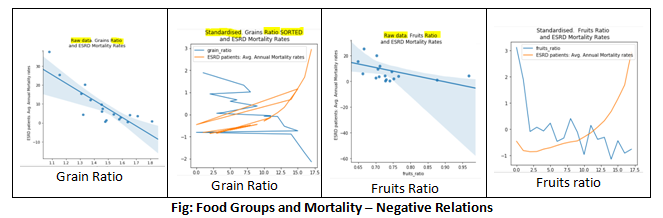
\includegraphics[scale=0.75]{result1}
\medskip 

\noindent Vegetables show positive (0.58) correlation i.e. mortality is high for the patients who took more vegetables. As the correlation is 0.58, hence, this is not a very strong conclusion. Data shows this correlation in older adults. Even though ratios of food intake amount to high end of recommended amounts (actual intake amounts also show positive relation) were used; age might have biased the correlation. This does not show conformity with the general recommendation to take more vegetables for CKD patients. However, as experiments with food subgroups show that vegetable subgroups such as Other vegetables (0.68), Red and Orange vegetables (0.55), and Starchy vegetables (0.44) show positive correlations that have an impact on the Vegetable group correlation.  Though more vegetable intake is a general recommendation for CKD patients; however, certain vegetables with more carbohydrates (and sugars) such as Starchy Vegetables as well as Vegetables with more Potassium and Calcium such as Tomatoes, and Spinach are recommended to take less. Considering the subgroups, the moderate positive correlation as this study found for vegetables food group is in conformity with the general recommendations for CKD patients.

\medskip 
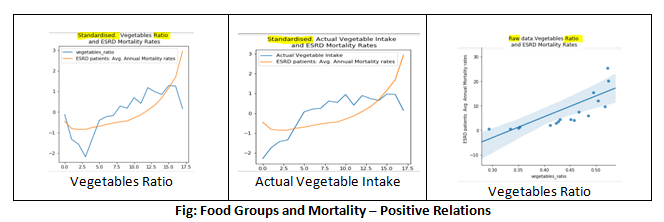
\includegraphics[scale=0.75]{result2}
\medskip 

\noindent \textbf{Food Subgroups and Mortality}


\noindent Experiments with aggregated (both NHANES and USRDS data) data to find associations between food subgroups and CKD mortality using PCA and Regression show that  Other vegetables (0.68),    Red and orange vegetables (0.55), and Starchy vegetables (0.44)  have positive correlations with mortality i.e. mortality is low when the intake amounts are low, and mortality is high when intake amounts are high. Data Exploration plots as given below also show the positive relations.

\medskip \medskip 
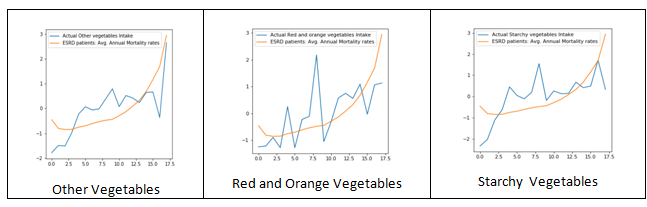
\includegraphics[scale=0.75]{result3}
\medskip  

\noindent  Food subgroups such as Alcoholic beverages (-0.79),    Added Sugars/Sugars and sweets (-0.64), Whole grains (-0.61), and  Nuts, Seeds, and Soy Products’ (-0.55) show the most negative correlations with CKD mortality. Data exploration also shows negative correlations as shown in the charts below. These outcomes can also be seen consistent with current knowledge except for Sugars. Prevalence of Stage 3 CKD is lower in Alcohol Drinkers than non-drinkers [2], Nuts being Phosphorous rich and Whole Grains being Potassium rich are detrimental to CKD patients and can cause higher mortality when taken more.
\medskip 

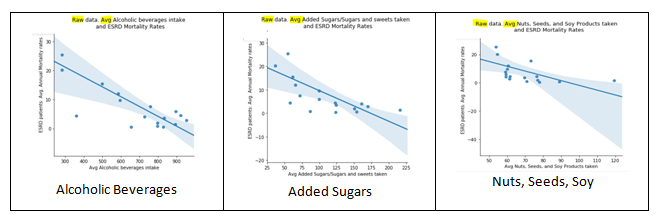
\includegraphics[scale=0.75]{result4}
\medskip 

\noindent \textbf{Mortality Study with non-aggregated Data}

\noindent Experiments where mortality rates based on ages were brought for each NHANES survey row (i.e. not aggregated), the following food subgroups show more positive correlations than others: Fats, Eggs, Other vegetables, Nonalcoholic beverages, White potatoes and Puerto Rican starchy vegetables, Tomatoes and tomato mixtures, Oils, Deep-yellow vegetables respectively. In the study the following subgroups showed more negative correlations than others: Grain mixtures, frozen plate meals, soups, Crackers and salty snacks from grain products, Milks and milk drinks, Sandwiches with Meat, Poultry, and fish, Poultry. Though the correlation numbers in this study are very low and negligible, however, the positive and negative correlations are consistent with current knowledge [48, 49, 50, 51, 52, 53, 54, 55, 56, 57].

\medskip  
\noindent \textbf{Food Groups, Food Nutrients, and Albumin Creatinine Ratio (ACR) Association}

\noindent The experiments using PCA and Regression showed negligible effect on ACR with food groups and subgroups. However, some food groups and/or nutrients such as Dairy, and  Sugars, Sweets, and Beverages’  have higher and positive though negligible (0.02) effect than the others where Fruits (-0.01) showed negative effect.  For nutrients, Poly unsaturated fatty acids (-0.02), and Iron (-0.02) have negative correlation where Choline (0.02) showed better positive correlation than others. Findings for Choline matches with medical knowledge [48]

\medskip 
\noindent As the correlations are not significant further analysis can be done on the data especially for food groups and nutrients that are found important (using PCA) in the data as provided below:


\medskip  
\noindent Dairy,  Fats, oils, and salad dressings’,  Fruits,  Grains,  Protein,   Sugars, sweets, and beverages’, Vegetables, Avg energy kcal,  avg protein gm,  avg carbohydrate gm,  avg total fat gm,  avg total saturated fatty acids gm, avg total monounsaturated fatty acids gm,  avg total polyunsaturated fatty acids gm, avg lutein zeaxanthin mcg,  avg thiamin vitamin B1 mg,  avg riboflavin Vitamin B2 mg,  avg Niacin mg, avg Calcium mg,  avg Phosphorus mg,  avg Magnesium mg,  avg Iron mg, avg Zinc mg,  avg Copper mg,  avg Sodium mg,  avg Potassium mg,  avg Selenium mcg,  Hexadecenoic gm,  Octadecenoic gm

\medskip 
\noindent \textbf{Food Subgroups and Albumin Creatinine Ratio (ACR) association}


\noindent The experiments showed  Milk desserts, Sauces, Gravies’ (0.22), and Alcoholic Beverages (0.087) have more positive correlations with ACR than the other food subgroups  i.e. taking more of these food subgroups results higher ACR values. Research by Uehara et al. [55] also shows that excessive Alcohol consumption can cause Proteinuria/Albuminuria (high ACR). Nettleton et al. [56] found that high fat dairy can be linked to high ACR values where low-fat dairy is not strongly linked to high ACR values. However, the correlation as this research found is very low. Low values might still explain a correlation where ACR values might depend on other factors in together than only these food subgroups. Fruits and juicy baby foods show negative correlation (-0.04) though not significant i.e. taking high amount does not increase ACR values that matched with current knowledge [57].

